\justifying

%%%%%%%%%%%%%%%%%%%%%%%%%%%%%%%%%%%%%%%%%%%%%%%%
\section{Introduction} \label{sec:intro}
%%%%%%%%%%%%%%%%%%%%%%%%%%%%%%%%%%%%%%%%%%%%%%%%

The remarkable technological progress attained in the last few decades has yielded significant benefits in the form of highly advanced imaging, spectroscopic, and polarimetric instruments designed for astronomical observations. These instruments have empowered us with the ability to scrutinize the Sun with exceptional detail. While some of these are ground-based telescopes, the others operate from space. Primarily, space-based instruments observe the Sun in Ultraviolet (UV), extreme ultraviolet (EUV), and X-ray bands, capturing radiation from upper atmospheric layers such as the transition region and corona, which emit due to their elevated temperatures. Various studies of the Sun over the last few decades have successfully uncovered the physical properties of the gas in the upper layers of the solar atmosphere using the observations recorded by X-ray imaging ({\it Hinode} X-ray Telescope \citep[{\it Hindoe}/XRT,][]{xrt}) and spectroscopy (the Spectrometer/Telescope for Imaging X-rays on {\it Solar Orbiter} \citep[{\it SO}/STIX,][]{stix}) and Extreme Ultraviolet (EUV) imaging (Atmospheric Imaging Assembly on the {\it Solar Dynamic Observatory} \cite[{\it SDO}/AIA,][]{aia}, Extreme ultraviolet Imaging Telescope on {\it Solar and Heliospheric Observatory} \cite[{\it SoHO}/EIT,][]{eit}, Solar Ultraviolet Imager on the {\it Geostationary Operational Environmental Satellites} \citep[{\it GOES}/SUVI,][]{suvi}, the Extreme Ultraviolet Imager on {\it Solar Terrestrial Relations Observatory-A} \cite[{\it STEREO-A}/EUVI,][]{stereo,euvi}, the Extreme-Ultraviolet Imager on {\it SO} \citep[{\it SO}/EUI][]{eui}) and spectroscopy \citep[Hinode/EIS,][]{eis}, among many others. The {\it Transition Region and Coronal Explorer} \citep[{\it TRACE},][]{trace}, the Solar Ultraviolet Measurements of Emitted Radiation on {\it SoHO} \citep[{\it SoHO}/SUMER,][]{sumer} and the {\it Interface Region Imaging Spectrograph} \citep[~{\it IRIS},][]{iris} allowed us to probe the chromosphere and the transition region in detail. These missions provide us with continuous full disk and Region of Interest (RoI) coverage of the Sun over the X-ray and EUV wavelengths. The situation is rather different in the Near-Ultraviolet (NUV) regime. There is clearly a lack of continuous coverage of the full solar disk in this wavelength range. 

One of the key challenges of carrying out solar observations in the UV regime from the ground is the strong attenuation by the Earth's atmosphere. One of the first stratospheric balloon-borne instruments was flown in 1970 and 1971 by \cite{herse79} to circumnavigate this. The instrument carried a 20 cm telescope that imaged the sun in 200{--}460 nm. The Rasolba balloon experiment was composed of a 30 cm telescope with an ultraviolet spectrograph. They obtained high-resolution spectra of the Sun in the spectral range 190 {--} 295 nm \citep{samain85,staath95}. Sunrise \citep{sunrise1,sunrise2} is a balloon-borne observatory that followed up these instruments to observe the Sun in the Near UltraViolet (NUV) regime with a telescope of 1 m diameter. It has flown twice, in June 2009 and June 2013, respectively and provided us with high-resolution imaging in 214, 300, 312, 388 and 397~nm with the Sunrise Filter Imager \citep[SuFI,][]{sufi} in 2009 and at 214, 279 and 397~nm in 2017 \citep{sunrise2}, Dopplergrams and vector magnetograms in \ion{Fe}{1} 525.02 nm with the Imaging Magnetograph eXperiment \citep[IMaX,][]{imax} at various locations on the solar disk.  During these two flights, along with quiet sun and active regions, Sunrise observed various solar phenomena, e.g. emerging flux events \citep{centeno17}, properties and dynamics of moving magnetic features around pores \citep{kaithakkal17}, proper motion of bright points in quiet sun and active regions \citep{jafarzadeh17}, properties of fibrils \citep{gaferia17} etc. These observations demonstrated the wealth of information this wavelength range carries and opened the path for full disk coverage of the Sun in the NUV.

The Solar Ultraviolet Imaging Telescope \citep[SUIT;][]{ghosh16,article} is one of the seven payloads onboard the Aditya-L1 mission \citep{adityal1, aditya} of the Indian Space Research Organization (ISRO), launched on September 2, 2023. The satellite is placed in a halo orbit around the Sun-Earth L1 point. With its eleven science bandpasses (eight narrow bands and three broad bands), {\suit} has the unique capability to probe different heights in the solar photosphere and chromosphere, helping us to understand various physical processes responsible for the transport of mass and energy from one layer to another. Moreover, SUIT provides the unique opportunity to measure the spatially resolved solar spectral irradiance in the NUV, which is central to our understanding of Sun climate relations. 

{\suit} is designed to continuously provide full-disk and RoI images of the Sun, with a 0.7{\arcsec} pixel size. It can track the RoIs while compensating for the differential rotation \citep{suit_algo}. Moreover, it can detect and localise flares with onboard intelligence and can automatically control the exposure time to avoid saturation. The main science questions that {\suit} aims to address are \citep[][]{suit_science,suit_main}: 

\begin{itemize}
    \item Coupling and dynamics of the solar atmosphere: {\it How is energy channelled and transferred from the photosphere to the chromosphere in the solar atmosphere?}
    \item Sun-Climate Relationship: {\it Understanding the Variability of Solar Spectral Irradiance (SSI) and NUV radiance of various features on the Sun.}
    \item Solar Flare Dynamics and Energy Distribution: {\it At Which wavelength Do flares emit the majority of their energy, and what proportion of this energy is from the NUV Range? What is the spectral energy distribution of flares?}
    \item Physics of eruptions at various spatiotemporal scales: {\it what physical processes drive eruptive phenomena observed at various spatiotemporal scales in the Photosphere and Chromosphere?}
\end{itemize}

In this work, we aim to forward model the observations recorded by {\suit} using the Max Planck Institute/University of Chicago Radiative Magneto Hydrodynamics \citep[MURaM,][]{muram} and MPS-ATLAS codes as well as observations recorded by the Interface Region Imaging Spectrograph (IRIS). MURaM is a three-dimensional (3D) MHD code designed to facilitate realistic simulations of magneto-convection and other related magnetic features (such as pores, sunspots and emerging flux) in the upper convection zone and photosphere. The simulation includes the effects of non-gray radiative transfer, partial ionization, full compressibility and open boundary conditions. The simulation gives us various physical quantities such as density, temperature, magnetic flux density etc. The MPS-ATLAS \citep{witzke12} code, which solves the radiative transfer equation varies rapidly with the help of opacity distribution functions, can be applied to the model atmosphere obtained from MURaM to synthesize the spectrum. Since the MURaM simulation cubes used here do not include the non-local thermodynamic equilibrium, these cannot be used to forward model the observations for chromospheric filter. Therefore, for this purpose, we utilize the observations recorded by~{\it IRIS} in \ion{Mg}{2} lines. {\bf The \ion{Mg}{2} h \& k lines, located at approximately 2803.5 and 2796.3~{\AA}, respectively, are among the most prominent spectral features in the near-ultraviolet (NUV) range. These lines are primarily formed in the upper chromosphere and the lower transition region \citep{leenarts13a, leenarts13b}, making them valuable diagnostics for studying chromospheric dynamics and heating. The Mg II lines exhibit core reversals due to non-LTE (local thermodynamic equilibrium) effects, providing insights into velocity flows, turbulence, and heating mechanisms in the solar atmosphere. Their strong sensitivity to temperature and density variations makes them particularly useful for investigating solar flares, where enhanced emission in these lines indicates energy deposition in the chromosphere.}

The rest of the {\bf chapter} is structured as follows. In \S\ref{sec:inst} we briefly describe details of the payload and present the effective area of various filter combinations. We present our method for calculating intensity maps from model atmospheres computed from MURaM, using MPS-ATLAS in \S\ref{sec:mps}. We present the measured point spread function (PSF) for the eleven science filters of {\suit} and the effects of the instrument PSF on the imaging in \S\ref{sec:psf} with the calculated intensity maps presented in \S\ref{sec:mps} and~{\it IRIS} observations. Finally, we summarize and conclude in \S\ref{sec:con}.

%%---------------------------------------------------
\begin{figure}
    \centering
    \includegraphics[trim={0.4cm 3.8cm 1cm 0cm},clip,width=0.85\textwidth]{optical_comp.jpeg}
    \caption[Transmission curves of various components of {\suit}]{Transmission as a function of wavelength of thermal filter (panel a), science filters (panels c and d), band pass filters (panel e) and the field corrector lens (panel f). We also plot the reflectivity of the mirrors in panel b and the quantum efficiency curve of the detector (panel g). Labels on x-axes are wavelength in nanometers.} 
    \label{fig:tras_prof}
\end{figure}
%%---------------------------------------------------
%%---------------------------------------------------
\begin{figure}
    \centering
    \includegraphics[trim={0cm 0cm 0cm 0cm},clip,width=0.85\textwidth]{eff_area.pdf}
    \caption{The effective area curves for all science filters as labelled.}
    \label{fig:eff_area}
\end{figure}
%%---------------------------------------------------

%%---------------------------------------------------
\section{The Instrument} \label{sec:inst}
%%---------------------------------------------------
The {\suit} is a two mirror off-axis telescope, which is designed to image the Sun with a plate scale of ~0.7{\arcsec}, and a field of view (FOV) of 0.75{\degree} on a 4096~$\times$~4096 charged coupled device (CCD), which has 12~$\mu$m pixel size. %Figure~\ref{fig:layout} shows a schematic diagram of the {\suit}. 
The entrance of the payload consists of an entrance door mechanism and a thermal filter(TF). The TF \cite[][]{thermal_filter_1, thermal_filter_2} is designed to cut down most of the incoming visible ($\approx$ 99.75\%) and infrared($\approx$ 99.5\%) radiation and transmits a very small fraction ($\approx$ 0.3\%) of the radiation within 200{--}400~nm. The transmitted light passes through the telescope and gets reflected from the primary and secondary mirrors, respectively, to arrive at the shutter mechanism, which is located between the secondary mirror and the filter wheels. For more details on the instrument, see \cite{article,suit_main}.


%%---------------------------%%
\begin{figure*}
    \centering
    \includegraphics[trim={2.7cm 6.7cm 2.7cm 4.5cm},clip,width=0.9\textwidth]{measured_psf.pdf}
    \caption{The measured PSF for the various filter combinations. The colourmap is area normalized, i.e. the sum of the PSF over the total area is unity.}
    \label{fig:psf_3d}
\end{figure*}
%%---------------------------%%

{\suit} has 11 science filters (first column Table~\ref{tab:science_filters}) and five bandpass filters (BPFs), which are used to keep the photon flux within the dynamic range of the CCD. Out of these five bandpass filters, while two are the spare copies NB08 and BB01, we designed three additional bandpass filters, namely, BP02, BP03 and BP04. These 16 filters are mounted on two filter wheels (FWs), each holding eight filters. The combination of the appropriate science filter and band pass filter is achieved by rotating the two filter wheels independently. Note that the secondary piece of BB01 is used as a combination of filter NB01 and BB01. Similarly, NB08 is combined with an identical NB08. Between the FWs and the detectors, a focusing lens is mounted on a piezo motor, which can be used as a focusing mechanism.  Fig.~\ref{fig:tras_prof} displays the transmission profile of the individual components in the optical path.

%%---------------------------%%
\begin{figure*}
    \centering
    %\hspace{-1cm}
    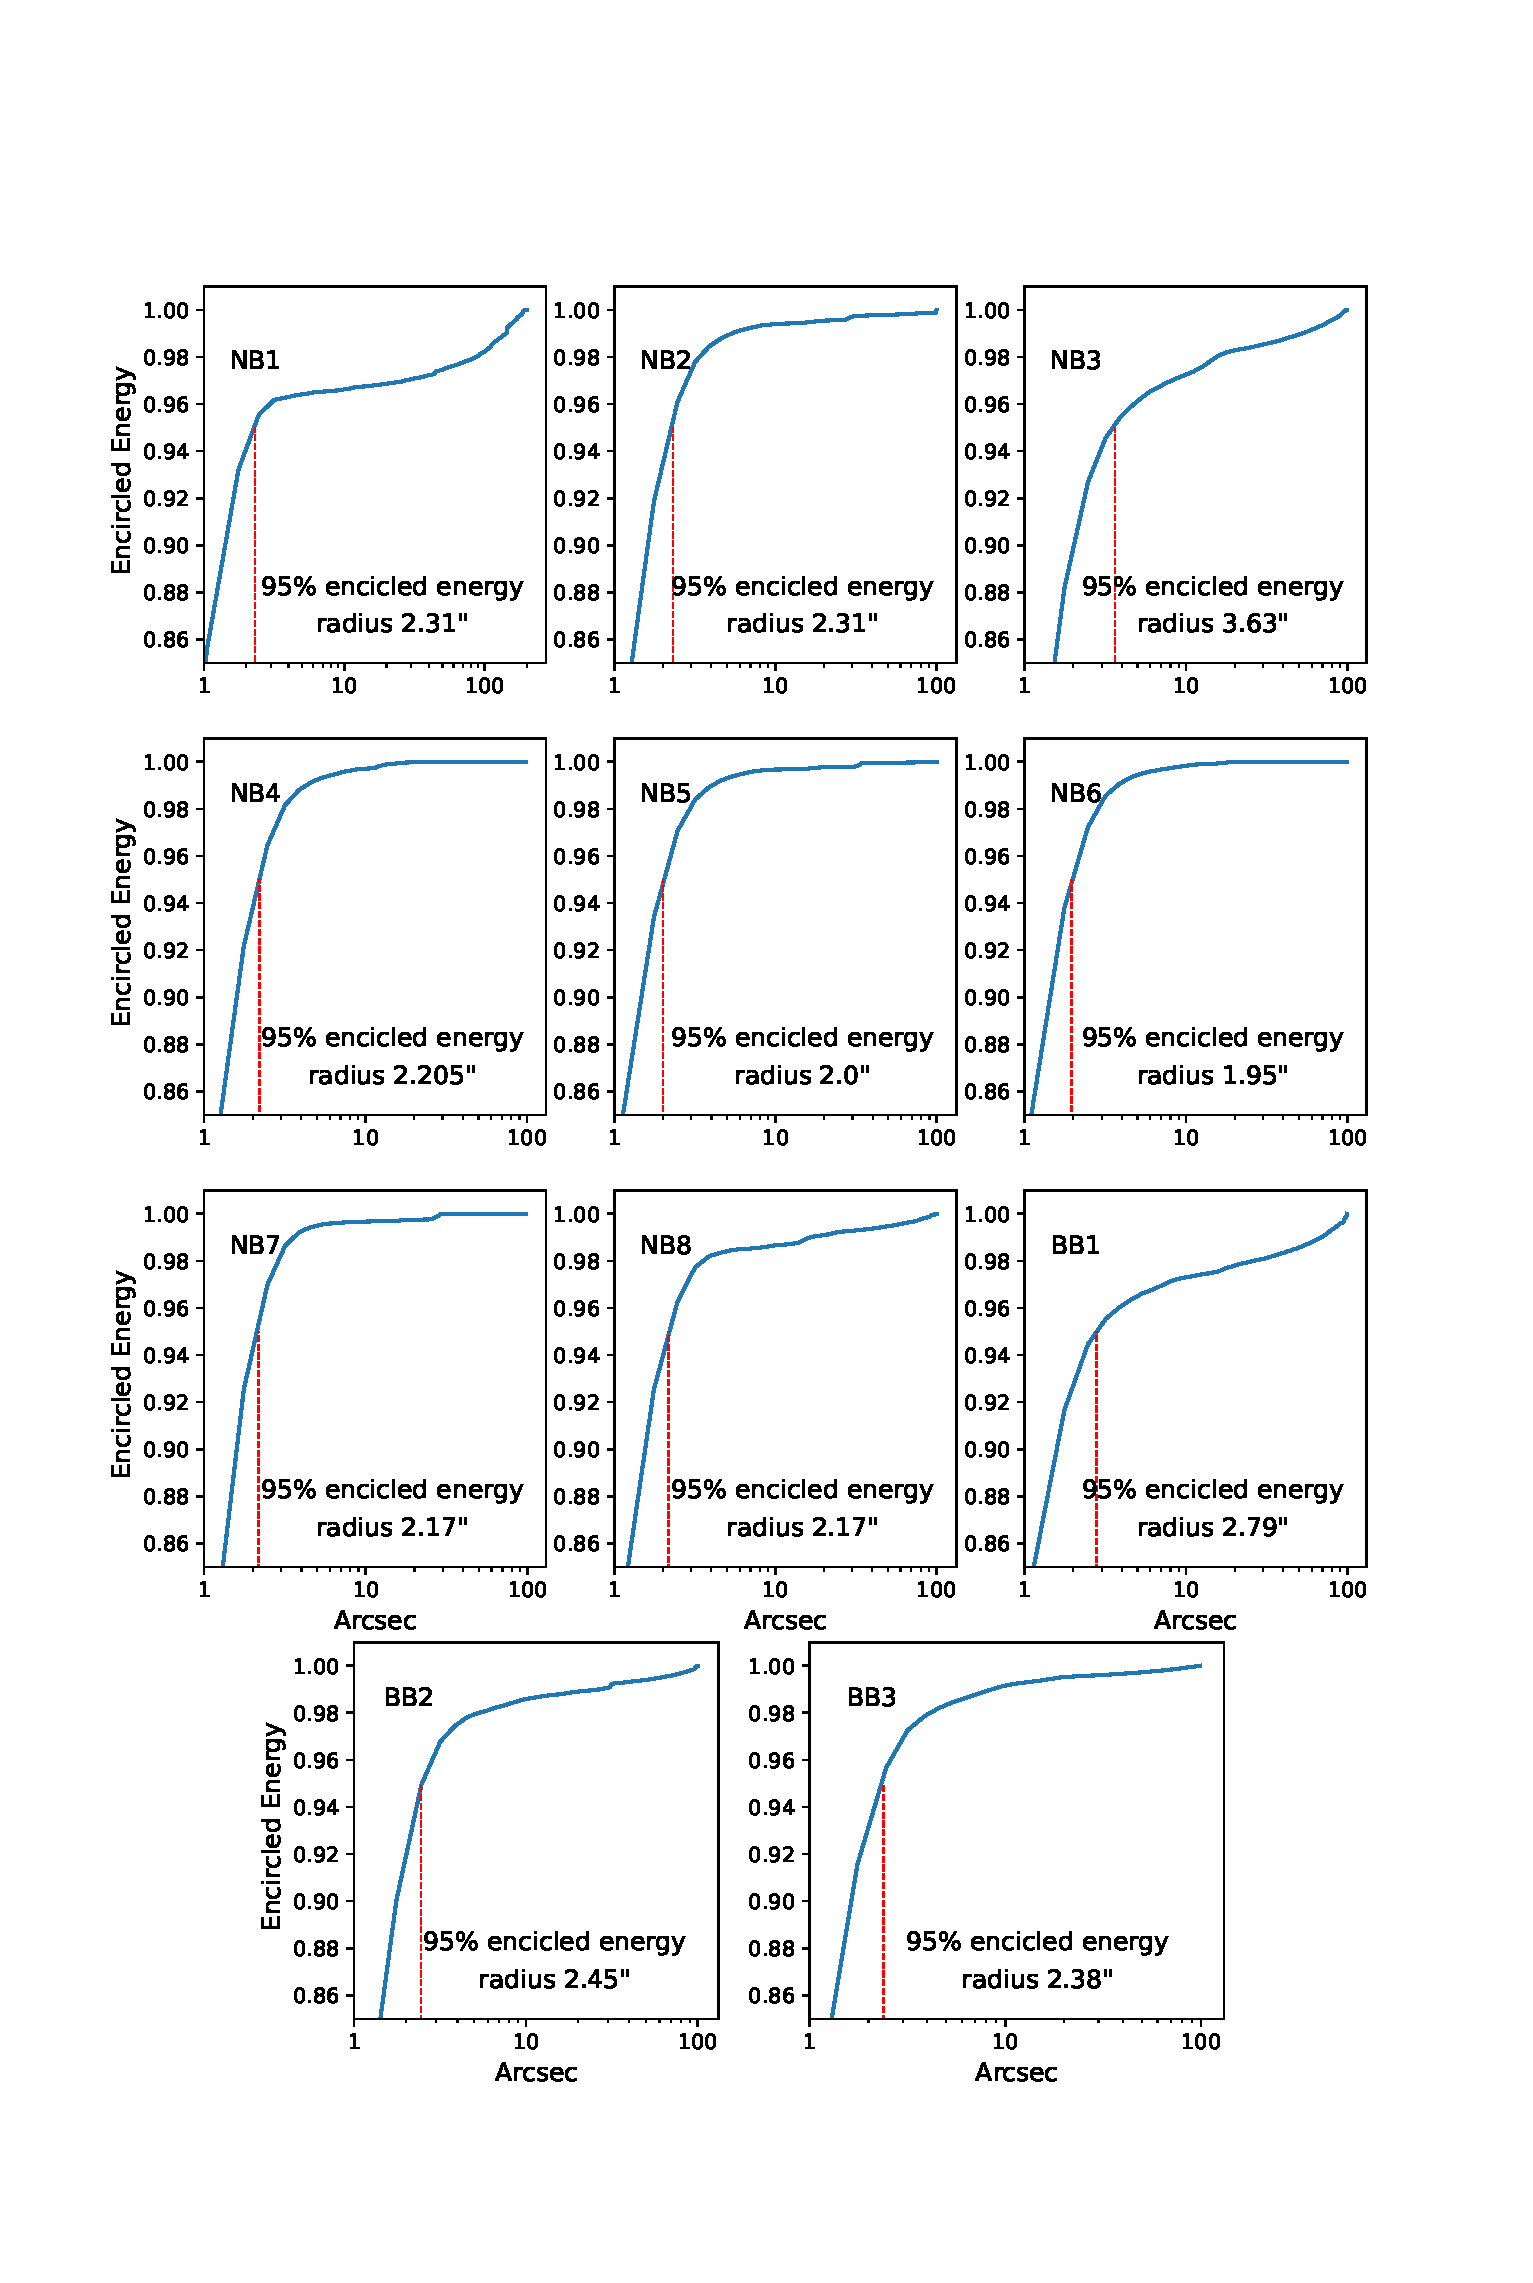
\includegraphics[trim={1.5cm 3cm 2.5cm 4cm},clip,width=0.85\textwidth]{psf_ese_2.eps}
    \caption{The encircled energy curve for the measured PSF. The 95\% encircled energy radius are marked with the vertical dashed red line. The angular scale of the 95\% encircled energy radius is also quoted in each panel for the specific filter combination.}
    \label{fig:psf_ese}
\end{figure*}
%%---------------------------%%

%%---------------------------------------------------
\subsection{Effective Area of SUIT}\label{eff_area}
%%---------------------------------------------------
Let $p(\lambda)$ be the incident photon flux on the entrance aperture. The photo-electron count at the detector, also known as Data Number (DN) is given by,

 $$   DN=\int~p(\lambda)~R(\lambda)~t~d\lambda $$

\noindent where $R(\lambda)$ is the instrument effective area for the specific filter combination and $t$ is the exposure time. The instrumental response, $R(\lambda)$, is computed by multiplying the measured response of all the optical components along the ray path. 

Hence,
    $$ R(\lambda)~=~TF(\lambda)\times PM(\lambda)\times SM(\lambda)\times SF_{i}(\lambda)\times $$
    $$ CF(\lambda)\times L(\lambda)\times QE(\lambda) \times A$$

\noindent where A is the entrance aperture area and TF($\lambda$), PM($\lambda$), SM($\lambda$), SF$_{i}$($\lambda$), CF($\lambda$), L($\lambda$) and QE($\lambda$) are the measured responses as a function of wavelength of thermal filter, primary mirror, secondary mirror, science filters, band pass filters, field corrector lens and the quantum efficiency of the CCD, respectively. The obtained effective area curves for each filter are shown in Fig.~\ref{fig:eff_area}. 

%%---------------------------------------------------------------
\begin{figure*}
    \begin{center}
        \begin{tikzpicture}[node distance=2cm]
            \node(muram)[io]{Model 3D atmospheres simulated by the radiative-MHD code MURaM};
            \node(slice)[io,right of=muram,xshift=3.5cm]{Slice the MURaM cubes and interpolate them to various $\mu$ values};
            \node(filter)[io,below of=muram,yshift=-1cm]{Use \suit~ science filter profiles accounting for all the optics on the ray path};
            \node(odf)[io,right of=filter,xshift=3.5cm]{Generate ODF tables for various filters using the MPS-ATLAS code};
            \node(rdt)[io,right of=odf,xshift=3.5cm,yshift=1.5cm]{Use ODF tables and 1D ray-atmospheres from the 3D MHD cube to carry out RT calculations using MPS-ATLAS};
            \node(int)[io,below of=rdt,yshift=-3.5cm]{Integrate the generated spectra for each pixel of the cube over the wavelength range of the filter profile to generate the intensity map};
            \node(conv)[io,left of=int,xshift=-4.5cm]{Convolve the total emergent intensity maps with relevant \suit~ PSF and bin to \suit~ plate scale to create mock observation};
            \draw[arrow](muram)--(slice);
            \draw[arrow](slice)--(rdt);
            \draw[arrow](filter)--(odf);
            \draw[arrow](odf)--(rdt);
            \draw[arrow](rdt)--(int);
            \draw[arrow](int)--(conv);
        \end{tikzpicture}
        \caption{The flow chart shows the entire process of generating the simulated intensity maps, from the data cubes and characterizing the filters.}
        \label{fig:flow}
    \end{center}
\end{figure*}
%%---------------------------------------------------------------

%%---------------------------------------------------------------
\subsection{The Point Spread Function (PSF) of {\suit}} \label{sec:psf}
%%-----------------------------------------------------------------
In Fig.~\ref{fig:psf_3d}, we plot the measured Point Spread Function (PSF) at the centre of the CCD for the different science filter combinations for {\suit}. The PSFs are highly peaked at the centre. The scattered light background becomes clearly visible due to the log scaling of the color bar and is more than two orders of magnitude lower than the peak.

Fig.~\ref{fig:psf_ese} shows the encircled energy curve for the measured PSFs for various filter combinations normalized to the total integral of unity. The vertical dashed lines in each plot show the radius within which 95\% of the incident light falls. For example, for the NB02 filter, 95\% of the incident light from a point source arrives within a 2.31{\arcsec} radius ($\sim$ 4.6{\arcsec} diameter) and 5\% of the light falls outside that region. Note that while the 95\% diameter is 4.6{\arcsec}, the PSF is strongly peaked. The overall diameter is considerably larger than the highly peaked part of the PSF because of the presence of a pedestal in the PSF. The pedestal is visible in all of the cases at the base of the central peak, although it is about 2 order of magnitude lower in all the cases (see Fig.~\ref{fig:psf_3d}). In some cases (e.g. NB01, BB02 etc.) a few or multiple smaller peaks apart form the pedestal are also visible. Similar radii for other filters are quoted in the corresponding panels of Fig.~\ref{fig:psf_ese}. The encircled count curves help us characterize the stray light for various filter combinations.

%%%%%%%%%%%%%%%%%%%%%%%%%%%%%%%%%%%%%%%%%%%%%%%%%%%%%%%%%%%%%%%%
\section{Forward Modeling SUIT intensity maps using MPS-ATLAS and MURaM} \label{sec:mps}
%%%%%%%%%%%%%%%%%%%%%%%%%%%%%%%%%%%%%%%%%%%%%%%%%%%%%%%%%%%%%%%%

One of the essential steps of characterizing the science filters was to conduct a thorough throughput modeling for the concerned filter combinations. However, quantifying the effects of the wavelength response of the optical components and the PSF on the spatially resolved observations, as well as the contrast variation, requires detailed modeling with resolved simulations of the Sun's surface. For this purpose, we use the MPS-ATLAS code. It is an updated version of the well established ATLAS9 \citep{atlas9} code that can efficiently generate Opacity Distribution Functions (ODFs), model atmospheres, and calculate emergent spectra in local thermodynamic equilibrium (LTE) for a given wavelength range by solving radiative transfer (RT) equation in plane parallel geometry using the assumptions of local-thermodynamic-equilibrium (LTE).

%%----------------------------------------------------------
\begin{figure}
    \centering
    \includegraphics[width=.85\textwidth]{mps.pdf}
    \caption{Forward modelled intensity maps at various $\mu$ values for BB02 filter of SUIT.}
    \label{fig:flux_maps}
\end{figure}
%%----------------------------------------------------------

%%----------------------------------------------------------
\begin{figure}
    \centering
    \includegraphics[trim={0cm 6cm 0cm 5cm}, clip, width=.85\textwidth]{mps_sim.pdf}
    \caption{Forward modelled intensity maps for various science filters of SUIT.}
    \label{fig:flux_maps_filt}
\end{figure}
%%----------------------------------------------------------

We use 3D MHD model atmospheres simulated by \cite{rempel20} and 1.5D RT with MPS-ATLAS \citep[see e.g.,][for details]{anusha21} with measured filter profiles of {\suit}, to calculate the emergent intensity. The 3D MHD simulation employs a symmetric lower boundary condition for the magnetic field and a variety of initial magnetic field configurations to create small-scale variations and various levels of magnetization. The RT equation is solved using the method of ODFs, accounting for both continuum and line opacities within the concerned wavelength range. This takes into account both continuum and line opacity within the concerned wavelength range. Accurately accounting for the line opacity is one of the major challenges in synthesizing spectra over a broad wavelength range. In the ODFs method, the opacity is sorted without the information of the corresponding wavelength within small intervals of wavelengths known as bins. The geometric mean of the sorted opacity values for multiple sub intervals within a given wavelength bin is pre-tabulated over atmospheric parameters such as temperature, pressure and micro-turbulent velocities. During RT calculations, opacity is then interpolated for the required grid parameters of the atmospheric model. The primary goal of the ODF method is to significantly minimize the computational time required for RT calculations. This becomes particularly crucial when computing emergent spectra across numerous atmospheres, such as those arising from 3D MHD simulations. 

\cite{anusha21} developed an optimized method using the MPS-ATLAS code that allows us to use an arbitrary filter profile instead of a rectangular filter profile. We use this method, with our measured effective area, to forward model intensity maps for NB01, NB02, NB05, NB06, NB07, BB01, BB02 and BB03 filter combinations that {\suit} is using.

We describe the end-to-end procedure in Figure~\ref{fig:flow}. The 3D MHD model atmospheres are sliced at various angles and interpolated to various Line of sight (LOS) angles. As described earlier, the ODF tables are generated for various atmospheric parameters, such as temperature, pressure and micro-turbulent velocities, for the measured science filter profiles. The generated ODF tables are used to solve the RT through the model atmosphere using the MPS-ATLAS code. This provides us the emergent intensity as a function of wavelength for all the rays of the model atmosphere. Integrating this intensity across the wavelength range, we determine the total emergent intensity for each filter.

Figure~\ref{fig:flux_maps} displays the {\suit}'s BB02 intensity maps obtained at various $\mu$ values, namely $\mu$~=~1.0, 0.8, 0.7 and 0.6, respectively. The spatial scale of the region is $(9~\textrm{Mm}\times9~\textrm{Mm})$ with $(512\times512)$ pixels, with a pixel size of $\simeq 0.025{\arcsec}/\textrm{pixel}$. This is at a much higher resolution than that of {\suit}, which is $\sim \textrm{0.7"/pixel}$. Moreover, these intensity maps do not include the effects of the instrument point spread function (PSF). Therefore,  we first need to convolve the computed intensity maps with the measured PSF of {\suit}, and then bin it to {\suit} plate scale to obtain synthetic observables that are comparable to {\suit} observations. Fig.~\ref{fig:flux_maps_filt} displays the simulated intensity maps for the {\suit} BB filters across the same MURaM cube.

We use the MURaM and MPS-ATLAS codes to forward model the observations for NB01, NB02, NB06, NB07, BB01, BB02 and BB03. We note that since the MURaM simulations studied here cannot be used for the chromospheric filters, namely NB03 (\ion{Mg}{2}~k), NB04 (\ion{Mg}{2}~h) and NB08 (\ion{Ca}{2}~k), we have used observations recorded by~{\it IRIS} to forward model the NB03 and NB04 filter observations.~{\it IRIS} also provides spectra corresponding to the continuum filter NB05. Hence, we forward model NB05, also using~{\it IRIS} observations. Forward modelling of SUIT observations using~{\it IRIS} data is straightforward as we do not need to use any MHD simulation cube and RT code. However, the convolution with the spatial PSF and the application of the spectral filter profile, etc. still must be carried out. For our analysis, we use dense raster scans from~{\it IRIS}. The dense rasters usually have $\sim$ 0.33{--}0.4 \arcsec per pixel spatial resolution. This spatial resolution is half of the pixel size of \suit. In addition to that, the 95\% encircled energy radius for most of the \suit~filter combinations is $\sim$ 2\arcsec. Hence, we can safely ignore the instrument characteristics of~{\it IRIS}. For the two filters where we are using~{\it IRIS} data, the bottom right box in Fig.~\ref{fig:flow} is replaced by~{\it IRIS} observations.

%%----------------------------------------------------------------------------
\begin{figure}
    \centering
    \includegraphics[trim={5cm 1cm 5cm 2.7cm},clip,width=0.85\textwidth]{BB3_convolve.pdf}
    \caption[The effects of convolution on the simulated BB03 intensity map]{The effects of convolution on the simulated BB03 intensity map. Panel a) MPS-ATLAS simulated BB03 intensity map. Panel b) convolved and binned BB03 intensity map. The normalized intensity variation along the horizontal and vertical black lines are plotted in panel c and d, respectively. The blue curves correspond to the simulated BB03 filter, whereas the orange curves correspond to convolved binned data.}
    \label{fig:BB3_conv}
\end{figure}
%%----------------------------------------------------------------------------

%%-------------------------------------------------------------------------
\subsection{{\suit} filters forward modeled with MPS-ATLAS}\label{sec:mps_contrast}
%%-------------------------------------------------------------------------

Following the procedure described above, we forward model the intensity maps in  NB01, NB02, NB06, NB07, BB01, BB02 and BB03. Since the spatial extent of the simulation box is much smaller compared to the size required to reliably convolve with the {\suit} PSF, we stitched the same simulated box multiple times to be able to convolve with the measured PSFs of SUIT. This could be done without problems due to the use of periodic boundary conditions in the MURaM simulation setup. Fig.~\ref{fig:BB3_conv}.a displays the stitched images obtained for BB03. In Fig.~\ref{fig:BB3_conv}.b, we display the corresponding image that is convolved with the PSF of the respective filter of SUIT and binned to its plate scale.

To compare the intensity contrast before and after the convolution, we plot intensity across a small part of the vertical (panel c) and a horizontal cut (panel d). The blue curves represent the intensity cut through the MPS-ATLAS simulated intensity maps, while the orange dashed curves are for convolved-binned intensity maps. The contrast variation across the cuts reproduces the intensity peaks and troughs in similar regions. These intensity cuts demonstrate that we can reproduce the intensity contrasts in the forward-modelled data with reasonably similar spatial positions. The forward-modelled observational features appear broader, with reduced contrast. This reduction in contrast, is anticipated given the difference in the plate scale of simulation and that of forward-modelled observations. The 95\% encircled energy is largely ~ 2{\arcsec} for most filter combinations (see Fig.~\ref{fig:psf_ese}). This would imply that the intensity from a point source would be redistributed to a circle of 2{\arcsec} radius. So, if we have two equally bright/dark point sources, they would be merged if the distance between them is 2{\arcsec} or less. Hence, we should be able to study contrast variation at the spatial scale of $\sim$ 2{\arcsec} using {\suit} observations. We have performed this exercise on all the filters corresponding to the photosphere and continuum and have obtained similar results.

%%----------------------------------------------------------------------------
\subsection{NB03 \& NB04}\label{sec:nb3_contrast}
%%----------------------------------------------------------------------------

As alluded earlier, to forward model NB03 and NB04 observations, we have used~{\it IRIS} archival data. The~{\it IRIS} obtains UV spectra with high spatial (0.33{--}0.4{\arcsec} per pixel), temporal (1s), and spectral resolution ($\sim$26 and $\sim$53~m{\AA}) and images of the scanned regions using the slit-jaw imager. In the spectral channels, the strongest lines that~{\it IRIS} regularly observes are \ion{C}{2}, \ion{Mg}{2} and \ion{Si}{4}. Here we use the very large and dense 320 step raster observation from 11th July, 2023 of a sunspot in AR 13363. The sunspot was located at the heliographic position of $\sim [-180\arcsec,-397\arcsec]$. The~{\it IRIS} raster had a FoV of $\sim [112\arcsec,175\arcsec]$. We use \textit{iris\_getwindata.pro} available in the \textit{sswidl} distribution to get the calibrated spectra over the raster FoV. This gives us the calibrated spectra for all the pixels in the raster FoV in units of $erg.cm^{-2}.s^{-1}.sr^{-1}.pix^{-1}$. We multiply the entire spectra of each pixel through the NB03 and NB04 effective area (see            
Fig.~\ref{fig:eff_area} panel b) and convolve with the measured PSF (see            Fig.~\ref{fig:psf_3d}) to forward model NB03, NB04 observations. Consequently, the observed intensity is, 

$$DN_{NB03}~=~\int~{\it IRIS}\_spec(\lambda)~R_{NB03}(\lambda)~t~d\lambda$$
and 
$$DN_{NB04}~=~\int~{\it IRIS}\_spec(\lambda)~R_{NB04}(\lambda)~t~d\lambda$$

\noindent where $R_{NB03}$ and $R_{NB04}$ are the measured effective area for the respective filter combinations. Fig.~\ref{fig:nb3_conv}.a shows the~{\it IRIS} raster FoV intensity map in the \ion{Mg}{2}~k line. The~{\it IRIS} image convolved with NB03 (NB04) PSF and binned to the {\suit} plate scale is shown in Figs.~\ref{fig:nb3_conv}.b(c).

To compare the intensity contrast obtained from SUIT images with those from~{\it IRIS} observations, in Figs.~\ref{fig:nb3_conv}.e \& f, we plot the normalized intensity profiles along the vertical (panel d) and horizontal (panel e) lines shown in panels a, b and c for NB03 and NB04 as labelled. The horizontal white dotted line encounters a light bridge on the western end of the sunspot (marked with a white arrow in Fig.~\ref{fig:nb3_conv} panels a, b \& c). We see three dips in the intensity profile in Fig.~\ref{fig:nb3_conv} panel e, as the horizontal white dotted line encounters the sunspot thrice. In both panels d \& e, NB03 (orange dashed line) and NB04 (black dot dashed line) has a lower contrast (peak to trough variation) compared to~{\it IRIS} (red solid line) and NB04 (black dot-dashed line) contrast. This is in line with our measurements of the PSF for NB03 \& NB04, as the measured PSF for NB03 has a higher scatter component in the background compared to NB04 (see panel c \& d in Fig.~\ref{fig:psf_3d}, Fig.~\ref{fig:psf_3d}). Therefore,  NB03 has a higher radius for 95\% encircled count (see NB03 and NB04 in Fig.~\ref{fig:psf_ese}). A higher radius for 95\% encircled count results in lower contrast in the convolved mock NB03 map.

%%%%%%%%-----------------%%%%%%%%%%%%%%%
\begin{figure}
    \centering
    \includegraphics[trim={5cm 0.6cm 6cm 0cm},clip,width=0.85\textwidth]{nb3_conv_edit.pdf}
    \caption[Effects of convolution on the~{\it IRIS} raster observation with the NB03 \& NB04 PSF]{Effects of convolution on the~{\it IRIS} raster observation with the NB03 \& NB04 PSF. Original (panel a), convolved with NB03 PSF and binned to {\suit} plate scale (panel b), convolved with NB04 and binned (panel c)~{\it IRIS} intensity maps obtained in \ion{Mg}{2}~k. Normalized intensity variation along the vertical-solid (horizontal-dashed) white line marked in panel a, b \& c are shown in panel d (panel e). Red-solid curves correspond to original~{\it IRIS} image, orange-dashed curves correspond to mock NB03 and black dot-dashed curves correspond to NB04.}
\label{fig:nb3_conv}
\end{figure}
%%%%%%%%-----------------%%%%%%%%%%%%%%%

%%-------------------------------------------
\subsection{NB05}\label{sec:nb5_contrast}
%%-------------------------------------------

The NB05 channel (with the central wavelength at 283.2~nm) is also observed by~{\it IRIS}. Therefore, we use the~{\it IRIS} 2832~{\AA} window observation of the same AR~13363 mentioned in \S\ref{sec:nb3_contrast}. %We use \textit{iris\_getwindata.pro} to get the spectra of the pixels in the raster FOV in units of $erg.cm^{-2}.s^{-1}.sr^{-1}.pix^{-1}$. Similarly, the whole spectrum is passed through the measured NB5 effective area and convolved with the measured PSF. 
In Fig.~\ref{fig:nb5_conv}.a, we plot the integrated intensity of the~{\it IRIS} 2832~{\AA} window. In panel b we plot the same region passed through the NB05 effective area and convolved and binned to {\suit} plate scale. In panels c and d we plot the normalized~{\it IRIS} intensity (red solid line) and normalized {\suit} NB05 intensity (orange dashed line) along the white dashed line and blue solid line marked in panels a and b, respectively. The features marked (`1' \& `2') in panels a and b are also marked in the normalized intensity variation panel e. Although there is a significant loss in contrast, the features are still identifiable. As demonstrated previously, various features are reproduced in the same spatial location with reduced contrast.

%%%%%%%%-----------------%%%%%%%%%%%%%%%
\begin{figure}
    \centering
    \includegraphics[trim={0.5cm 0.2cm 2cm 0cm},clip,width=0.85\textwidth]{NB5_feature_1.pdf}
    \includegraphics[trim={2.7cm 0.2cm 3cm 2cm},clip,width=0.95\textwidth]{NB5_feature_2.pdf}
    \caption[Effects of convolution on the~{\it IRIS} raster observation with the NB05 PSF]{Effects of convolution on the~{\it IRIS} raster observation with the NB05 PSF. We plot the~{\it IRIS} raster intensity map obtained in 2832~{\AA} continuum in panel a and the convolved-binned intensity image in panel b. 
    The normalized intensity variation obtained from both images along the white-dashed and blue-solid lines are shown in panels c and d, where red solid lines correspond to the original~{\it IRIS} image and orange dashed lines correspond to the convolved-binned intensity map. The two thin features marked by `1' and `2' within the sunspot in panels a and b are also marked in the intensity variation plot.}
\label{fig:nb5_conv}
\end{figure}
%%%%%%%%-----------------%%%%%%%%%%%%%%%

We have also used a very large, dense 320-step raster observation from 20th July 2023 of a sunspot in AR 13376 to create the mock observation. The sunspot was located at the heliographic position of $\sim [-147",325"]$. The~{\it IRIS} raster had a field of view (FoV) $\sim [112",119"]$. As described earlier, we forward modeled SUIT observations in the NB05 passband for this region. In Fig.~\ref{fig:nb5_conv_1} panel a we plot the integrated map obtained in~{\it IRIS} 2832~{\AA} window. In panel b we plot the same region passed through the NB05 effective area and convolved-binned to the {\suit} plate scale. In panel c(d) we plot a cropped view of the sunspot in the southern part of the region in~{\it IRIS} 2832~{\AA} ({\suit}~NB05 convolved). The light bridge within this sunspot narrows in thickness as we move from the upper-left to the lower-right. We take multiple measurements close to one another and average them to calculate the thickness of the light bridge at some specific location. In the northern part, the lightbrdge is $\sim 2\arcsec$ thick in the~{\it IRIS} observation and 4$\arcsec$ in the mock NB05 observation (see upper set of white arrows in panels c and d). It narrows down to 1$\arcsec$ in the southern part in the~{\it IRIS} observation, and 1.8$\arcsec$ in the mock NB05 observation (lower set of white arrows).

We take a slice through the sunspot and the light bridge, marked with a vertical white line in Fig.~\ref{fig:nb5_conv_1} panel c. The intensity along this line for normalized~{\it IRIS} contrast (solid red line) and convolved NB05 contrast (dot-dashed blue line), is plotted in Fig.~\ref{fig:nb5_conv_1} panel e. The light bridge is marked with a black arrow in the intensity profile.

%%%%%%%%-----------------%%%%%%%%%%%%%%%
\begingroup
    \centering
    \includegraphics[trim={3cm 4cm 3cm 0cm},clip,width=0.85\textwidth]{suit_sunspot_part1.pdf} \\
    \includegraphics[trim={1cm 0.2cm 1cm 1cm},clip,width=0.85\textwidth]{suit_sunspot_contrast_2.pdf}
    \captionof{figure}[Effects of convolution on the~{\it IRIS} raster observation with the NB05 PSF]{Effects of convolution on the~{\it IRIS} raster observation with the NB05 PSF. Panel (a):~{\it IRIS} raster intensity in 2832~\AA\ continuum.A large sunspot with a thin, light bridge in the middle is present in the southern part of the region. Panel (b): The~{\it IRIS} raster observation in panel a convolved with the NB05 PSF (see fig.~\ref{fig:psf_3d} panel e). Panel (c) \& (d): Zoomed view of the larger sunspot in the South in~{\it IRIS} and the simulated \suit\ NB05 map, respectively. The light bridge in the middle of the sunspot is marked by a set of four white arrows. The thickness of the light bridge at two locations is marked in both the panels. The normalized intensity along the vertical  white line drawn in panel (c) is plotted in panel (e). The normalized intensity of the original~{\it IRIS} (mock NB05) observation is plotted in solid red (dot-dashed blue) line. The light bridge is marked in the intensity profile with a black arrow.}
    \label{fig:nb5_conv_1}
\endgroup
%%%%%%%%-----------------%%%%%%%%%%%%%%%

%%%%%%%%%%%%%%%%%%%%%%%%%%%%%%
\section{Summary and Conclusions}\label{sec:con}
%%%%%%%%%%%%%%%%%%%%%%%%%%%%%%

The observation of any optical telescope is convolved by the PSF of the telescope. The PSF represents the response of the optical system to a point source. It quantifies the extent of blurring of a point source when imaged through the optical system, as well as the effects of various components like scattering, diffraction, etc. We have applied the measured PSF at the \suit\ detector plane for various filter combinations to the emergent radiation from MURaM simulation cubes (computed by MPS-ATLAS) and to pre-existing~{\it IRIS} observations to create mock {\suit} observations. The {\suit} PSF in all of the filter combinations is highly peaked with a pedestal $\sim$ two orders of magnitude lower (see Fig.~\ref{fig:psf_3d}). In most of the filter combinations the 95\% encircled count radius is $\sim$ 1.4 {--} 2.5{\arcsec}. This would imply that two equally bright or dark features on the Sun $\sim$ 2{\arcsec} apart would be merged in the corresponding {\suit} observation. Hence, we could resolve features on a spatial scale of $>$ 2.5{\arcsec} for the corresponding filters in {\suit} observations. These projections are more relevant for line filters in {\suit} (e.g. NB03(\ion{Mg}{2} k), NB04(\ion{Mg}{2} h, NB08 (\ion{Ca}{2} h)), as it would exhibit more features in close proximity (bright points in ARs and QS, the plage regions around sunspots, small eruptions in ARs). These projections are made with the measured PSF at the center of the CCD. The PSF distortions increase gradually as we move away from the centre of the CCD, with more angular elongation. 

We believe the forward modeling pipeline will help us simulate {\suit} observations from existing MHD simulations and compare them to real {\suit} observations to constrain current model parameters. The comparisons with forward-modelled mock {\suit} observation with real {\suit} observations over time would also provide useful insights into the degradation of the instrument with respect to the on-ground projections. The deconvolution algorithm would be useful to improve the contrast across {\suit} observations and spatially localize features more reliably on the solar surface.